\chapter{Servizio}
\label{chap:serv}
In questo capitolo verranno esposti in dettaglio l'architettura finale dell'applicativo sviluppato che permette la comunicazione tra il Surface Dial e la pagina web, le funzionalitá implementate grazie al suddetto servizio, una breve descrizione per lo sviluppatore che intederá utilizzarlo e i test implementati attraverso MSTest con lo scopo di verificare il corretto funzionamento del software
\section{Architettura Software}
Il progetto sviluppato si presenta suddiviso in due parti ben distinte:
\begin{itemize}
\item \textbf{Servizio Angular}
\item \textbf{Applicazione UWP}
\end{itemize}

\subsection{Servizio Angular}

In Angular, i Servizi rappresentano un tassello fondamentale per la realizzazione di un'applicazione. Un servizio è solitamente rappresentato da una classe indipendente dalla View che viene definita per svolgere un compito ben preciso ed effettuare delle operazioni strettamente correlate tenendo in mente il principio di singola responsabilità.\\
È possibile definire più servizi all'interno di un'applicazione, ognuno dei quali si occupa di portare a termine un determinato incarico incrementando la modularitá del progetto, inoltre un servizio puó a sua volta dipendere da altri servizi, che vengono definiti nel costruttore del servizio stesso.\\

Avvalendosi di Angular CLI, possiamo creare un Servizio tramite il comando:

\vspace{1.0cm}
\begin{lstlisting}[caption={Esempio creazione servizio},style=javaScriptCode]
	ng generate service <nome-del-servizio> <flag-opzionali>
\end{lstlisting} 
\vspace{1.0cm}
Una volta creati, i servizi possono essere iniettati all'interno di uno o più componenti grazie al meccanismo di \emph{Dependency Injection}.\\

Per poter utilizzare un servizio da noi definito, dobbiamo registrarlo con uno degli Injector presenti in Angular. Esiste infatti una gerarchia di Injector, che Angular provvede a creare, alla base dei quali c'è il cosiddetto Root Injector, che viene creato in fase di bootstrap dell’applicazione e i servizi registrati con quest’ultimo sono disponibili per tutta l’applicazione.\\

Per ogni Injector esiste sempre una sola istanza di un determinato servizio, come specificato nella documentazione ufficiale:\\

\emph{"Services are singletons within the scope of an injector. That is, there is at most one instance of a service in a given injector."}\\

L’ Injector si occupa di creare le dipendenze e si serve di un Provider, un oggetto il quale indica all'Injector come ottenere o creare un'istanza di una dipendenza.
Per ogni dipendenza che si vuole usare nell'applicazione si deve registrare un provider con un Injector, in modo che quest'ultimo possa poi utilizzare il provider per creare nuova istanza di quella dipendenza.

\subsubsection{Singleton services}

Per restare in linea con le direttive utilizzare dal gruppo Loccioni nello sviluppo dei loro servizi, abbiamo utilizzato il forRoot() pattern per l’injection del servizio nell’applicazione.\\

Questo pattern permette di specificare un modulo personalizzato per il servizio, il quale contiene un metodo statico chiamato appunto forRoot() che restituisce un ModuleWithProvider parametrizzato al modulo del Servizio.\\

Questo pattern permette di effettuare l’import del modulo nell’AppModule richiamando il metodo forRoot(), cosi da non dover appesantire il Provider del modulo iniziale e in linea di principio é bene utilizzarlo quando un provider prende in ingresso dei parametri, così da non dover specificarli ogni qualvolta il modulo venga utilizzato.

\subsubsection{DialService}

Lo scopo finale del servizio che abbiamo implementato é quello di poterlo utilizzare come ponte o intermediario tra il Surface Dial, che si interfaccia nativamente con l'applicazione UWP, la quale contiene una WebView con all'interno caricata una pagina custom Loccioni, e i componenti della View all'interno della pagina che intendono utilizzare il servizio.\\

Il componente che dipenderá da questo determinato servizio, chiamato appunto DialService, potrá facilmente utilizzare le funzionalitá messe a disposizione dal Surface Dial e interpretare gli eventi intercettati a RunTime.\\

Il core del servizio implementato è rappresentato dalla Classe DialService, essa infatti si occupa di inizializzare il servizio e rendere disponibile la comunicazione bi-direzionale tra il lato Web e quello UWP.In particolare si occupa di recuperare l'oggetto C\# iniettato a sua volta dentro l'oggetto window della pagina web, con visibilitá globale.\\

\vspace{1.0cm}
\begin{lstlisting}[caption={Recupero oggetto C\#},style=javaScriptCode]
	this.dial = (window as any).dial;
\end{lstlisting} 
\vspace{1.0cm}

L'oggetto dial viene poi inserito per questioni di sicurezza in una classe DialProxy, la quale implementa a sua volta l'interfaccia da noi sviluppata DialBackendBridge, nella quale sono presenti tutte le funzionalitá dell'oggetto "dial", richiamabili quindi da Web.

\subsubsection{DialBackendBridge}

DialBeckendBridge rappresenta l'interfaccia contenente la dichiarazione dei metodi implementati nella classe DialController dell'applicazione UWP.\\
In questo modo, tramite l'oggetto dial iniettato, sará possibile richiamare a RunTime i metodi dichiarati nel C\# attraverso il Web.\\

\vspace{1.0cm}
\begin{lstlisting}[caption={Interfaccia DialBackendBridge},style=javaScriptCode]
export interface DialBackednBridge{
		
	getProductId(): string;
	
	setMenu(arrayOfItem: any[]): void;
	
	clearMenu(): void;
	
	deleteItem(tag: string): void;
	
	addItem(item: any): void;
	
	createDialMenuItem(tag: string, displayText: string, icon: string): any;
	
	setDefaultItem(defaultItems: string[]): void;
	
	manualInvoke(tag: string): void;		

}		
\end{lstlisting} 
\vspace{1.0cm}

\newpage
\subsubsection{DialFrontendBridge}

Per rendere questa comunicazione bi-direzionale, abbiamo creato una classe DialFrontendBridge con la responsabilitá di rendere visibili dei metodi all'interno dell'oggetto window e quindi richiamabili tramite script dall'applicazione UWP.\\

L'invocazione di questi metodi comporta la successiva emissione di un determinato evento a coloro che vi si sottoscrivono, con la possibilitá del passaggio di parametri di tipo stringa.\\

Tramite l'utilizzo degli EventEmitter messi a disposizione dal core di Angular e definiti come mostrato nel codice sottostante, la classe DialFrontendBridge permette all'utilizzatore del servizio di sottoscriversi a determinati eventi pubblici, che quando richiamati emettono un determinato valore.\\

\vspace{1.0cm}
\begin{lstlisting}[caption={EventEmitter esposti da DialFrontendBridge},style=javaScriptCode]
public onRotationEvent = new EventEmitter<{tag: string, degree: string}>();
public onPressedRotationEvent = new EventEmitter<{tag: string, degree: string}>();
public onClickEvent = new EventEmitter<string>();
public onInvokeEvent = new EventEmitter<string>();
public onScreenContactStartedEvent = new EventEmitter<{x: string, y: string}>();
public onScreenContactContinuedEvent = new EventEmitter<{x: string, y: string}>();
public onScreenContactEndedEvent = new EventEmitter();
\end{lstlisting} 
\vspace{1.0cm}

Affinché questi metodi possano essere richiamati tramite script dall'applicazione UWP é stato necessario inserire l'istanza della classe all'interno dell'oggetto window, cosi da renderlo visibile e utilizzabile dall'esterno.\\

\vspace{1.0cm}
\begin{lstlisting}[caption={Inserimento DialFrontendbridge in window },style=javaScriptCode]
(windowa as any).DialFrontendBridge = this.dialFrontendbridge;
\end{lstlisting} 
\vspace{1.0cm}

\newpage
\vspace{1.0cm}
\begin{lstlisting}[caption={Metodi esposti DialFrontendBridge},style=javaScriptCode]
    public RotationEvent(tag: string, degree: string): string{
        this.onRotationEvent.emit({tag, degree});
        return degree;
    }
    public PressedRotationEvent(tag: string, degree: string): string{
        this.onPressedRotationEvent.emit({tag, degree});
        return degree;
    }
    public ClickEvent(tag: string){
            this.onClickEvent.emit(tag);
    }
    public InvokeEvent(tag: string){
        this.onInvokeEvent.emit(tag);
    }
    public ScreenContactStartedEvent(x: string, y: string){
        this.onScreenContactStartedEvent.emit({x, y});
    }
    public ScreenContactContinuedEvent(x: string, y: string){
        this.onScreenContactContinuedEvent.emit({x, y});
    }
    public ScreenContactEndedEvent(){
        this.onScreenContactEndedEvent.emit();
    }
\end{lstlisting} 

\subsubsection{Widget}

Un widget Aulos è un componente in esecuzione all’interno di una DashBoard con lo scopo di rappresentare o modificare i dati ottenuti dal backend collegato fisicamente ad una macchina.\\

Nella nostra applicazione abbiamo modificato degli Widgets giá esistenti del gruppo Loccioni, utilizzando all'interno di essi il nostro servizio \emph{DialService}, con lo scopo di renderli controllabili attraverso il Dial. Siamo partiti tentando di agganciarsi ad un semplice Widget che visualizzasse un range di possibili valori rappresentato da uno \emph{slider grafico} e da un \emph{Radial Gauge}, con l'intento di variare, anche solo graficamente, il valore corrente attraverso l'evento rotazione del Dial.\\

\begin{lstlisting}[caption={Sottoscrizione evento rotazione},style=javaScriptCode]
if (this.widget.runMode){
  if (this.dialService.isDialConnected){
	this.createMenuVoice();
	this.dialService.dialFrontendBridge.onRotationEvent.subscribe(
	({tag, degree}) => {
	  if (tag === this.id){
		this.value += (parseInt(degree, 10) * 5);
		this.changeDetectorRef.detectChanges();
	  }
	});
  }
}
\end{lstlisting} 

Successivamente, abbiamo creato un Widget chiamato ChannelDialWidget, un widget contenente al suo interno, al contrario di quelli sopra citati, il collegamento a \emph{N} diversi canali collegati ad un endopoint nel backend, permettendo non solo la lettura, ma anche la modifica effettiva della persistenza dei dati.
Questo ci ha permesso di sviluppare delle funzionalità custom per quel determinato Widget al fine di poterne acquisire il controllo, e scegliere canale per canale, il valore da settare, permettendo la variazione non solo grafica ma anche effettiva dei dati mostrati.\\

Per rendere sicure queste funzionalità abbiamo previsto la variazione grafica dei valori con la singola rotazione e la successiva modifica lato backend solamente qualora il dial venga premuto, altrimenti attraverso la funzionalità combinata di pressione e rotazione, così da evitare una involontaria modifica nel momento della presa possesso del widget o nella fase di transizione tra l'acquisizione su schermo e il successivo utilizzo su un piano di lavoro.\\

Analogamente all'evento sopra mostrato, chiamato onRotationEvent, gli eventi al quale il widget ChannelDialWidget si sottoscrive al fine di variare i valori di un canale selezionato, sia graficamente che in modo permanente lato backend, sono i seguenti:

\begin{itemize}
\item \emph{onRotationEvent} 
\item \emph{onClickEvent} 
\item \emph{onPressedRotationEvent}
\end{itemize}

Durante la sua inizializzazione, il widget si sottoscrive all'evento di Invoke, con lo scopo di intercettare il tag sul quale viene richiamato il medesimo metodo dal Dial. Successivamente, se l'evento invoke richiamato restituisce il tag corrispondente all'ID del Widget in ascolto, viene pulito il menu del dial e vengono caricate le voci di menu inerenti ai canali collegati a quel determinato Widget cosi da poter essere richiamati e intercettati a loro volta dalla sottoscrizione all'evento onInvokeEvent.
 
\subsection{Applicazione UWP}

Il secondo componente del progetto è costituito da un'applicazione UWP (Universal Windows Platform), presa in considerazione poiché la più recente tra i framework Microsoft e tra le sue caratteristiche troviamo la sicurezza e la portabilità tra le diverse piattaforme Windows, ciò consente un maggiore supporto nel tempo e intercambiabilità tra i dispositivi dove utilizzarla. L'eseguibile sviluppato prende il nome di \textbf{DialBridge}.\\

\subsubsection{DialBridge}

L’applicazione DialBridge ha come responsabilità quella di comunicare con il Dispositivo HID attraverso le librerie fornite da Microsoft e allo stesso tempo comunicare con la pagina Web contenuta al suo interno.\\

Inizialmente abbiamo creato un'unica soluzione contenente sia la WebView che il Core dell'applicazione, ma abbiamo riscontrato un problema nell’injection dell'oggetto utilizzato per la comunicazione Web-UWP, poichè esso deve necessariamente essere iniettato a runtime.\\

Di conseguenza abbiamo creato due diverse soluzioni:

\begin{itemize}
\item \textbf{Core:} Contiene il nucleo dell’applicazione.
\item \textbf{EmbeddedBrowserView:} Contiene la parte runtime del progetto\\ che 			effettua l’injection dell’oggetto nella pagina Web.
\end{itemize}

\subsubsection{Core}

Nel Core è contenuta la parte del progetto UWP che non richiede l'avvio a runtime e comprende le seguenti classi:

\begin{itemize}
\item DialController
\item WebNotifier
\item DialMenuItem
\end{itemize}

\subsubsection{DialController}

La classe DialController è una tra le più importanti poiché una sua istanza verrà poi inserita all’interno della WebView e servirà al servizio DialService per la comunicazione Web-UWP. I metodi pubblici al suo interno sono gli stessi dell’interfaccia DialBackendBridge che vengono utilizzati appunto tramite l’oggetto iniettato inizialmente.\\

Al suo interno troviamo un’ istanza della classe RadialController, ovvero la libreria Microsoft che permette la manipolazione del Dial, un'istanza di RadialControllerConfiguration e infine un notifier.\\

Nel costruttore abbiamo assegnato agli eventi presenti nella classe RadialController il relativo handler nella classe WebNotifier, in questo modo ogni volta che verrà emesso un determinato evento la pagina web riceverà una notifica e verrà svolta la funzione associata a quella determinata voce di menù.

\subsubsection{WebNotifier}

La classe WebNotifier contiene al suo interno una istanza della WebView ed ha come responsabilità quella di fornire i metodi che verranno poi utilizzati come EventHandler per gli eventi forniti dalla classe RadialController, in modo tale da riuscire a comunicare, attraverso la WebView al suo interno, alla pagina web l’emissione dell’evento stesso.\\

Al suo interno è presente anche un oggetto della classe CoreWindow utilizzato per spostare la posizione del mouse sullo schermo al primo contatto del Dial sulla superficie.

\subsubsection{DialMenuItem}

La classe DialMenuItem è una classe “modello” utilizzata per rappresentare un elemento contenuto nel Menu del Dial.

\subsubsection{MainPage}

Nella Main Page avviene l’inizializzazione dei componenti RadialController e la navigazione alla pagina web desiderata.\\

All’interno del metodo NavigationStarting troviamo il metodo AddWebAllowedObject che ci permette, di iniettare l’oggetto della classe DialController durante il caricamento, passandogli come parametri una stringa rappresentate il nome dell'oggetto, con il quale potrá essere intercettato lato Web e l'istanza dell'oggetto da iniettare.

\begin{lstlisting}[caption={Injection oggetto C\#},style=javaScriptCode]
webView.AddWebAllowedObject("dial", dial);
\end{lstlisting}

\section{Posizionamento su schermo}

Uno dei maggiori vantaggi dell’utilizzo di un surface Dial è la possibilità di posizionarlo sopra uno schermo compatibile e di variare il suo funzionamento in base alla posizione utilizzata.
Questa funzionalità è gestita dal sistema operativo e comunica solamente con elementi nativi UWP e con  display touch-screen compatibili ( Surface Pro 4/6/7 e Sruface Studio).

\begin{figure}[htpb!]
  \centering
  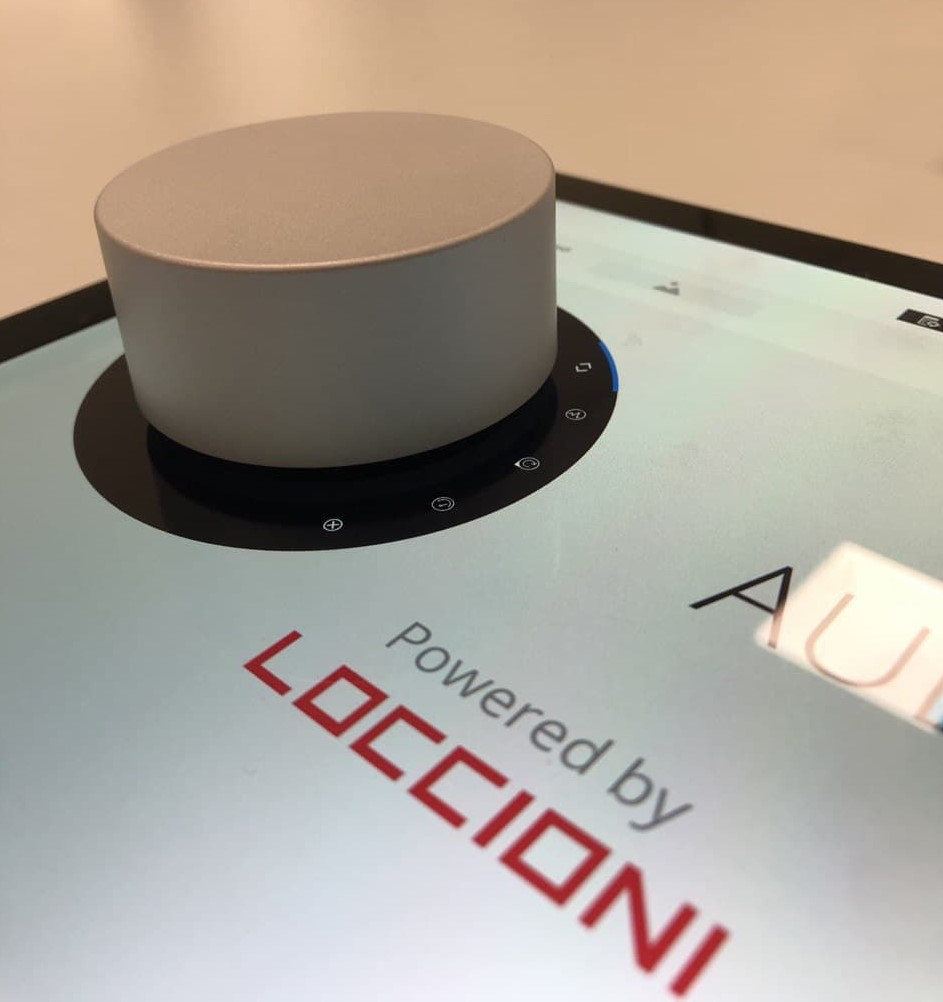
\includegraphics[width=0.5\textwidth]{DialSchermo}
  \caption{Microsoft Dial posizionato sopra un surface pro 6}
\end{figure}
Inizialmente abbiamo preso in considerazione la possibilitá di suddividere il layout dell’applicazione nativa in N riquadri, all’interno dei quali avremo posizionato il relativo Widget da controllare. Questa soluzione presentava peró delle limitazioni, in quanto in base alla risoluzione del dispositivo utilizzato, i widget caricabili in ogni riquadro del layout erano limitati al numero di riquadri definiti dall'applicazione UWP.\\
Abbiamo quindi cercato una soluzione, che spostasse la responsabilitá di acquisire il posizionamento lato Web anziché lato UWP, implementando una soluzione che ci permettesse di avere un numero variabile di Widget configurabili nella Dashboard e la successiva acquisizione di essi.\\

Analizzando gli eventi richiamabili dalla classe RadialController, in particolare quelli inerenti al contatto con lo schermo, abbiamo notato che prendevano come parametro in ingresso un oggetto di tipo \emph{RadialControllerScreenContact} fornitogli dalla Libreria. 
Questo oggetto possiede due attributi relativi al Posizionamento ( Position ) e al Bound ( Bounds ) dall'area del rettangolo generato dal Dial sullo schermo.

Grazie all’attributo Position di tipo Point, é possibile ottenere, attraverso le coordinate X e Y, il punto centrale nel quale il Dial é posizionato.

\vspace{1.0cm}
\begin{lstlisting}[caption={Metodo ScreenContactStartedAsync},style=javaScriptCode]
 internal async Task ScreenContactStartedAsync(
 	RadialControllerScreenContactStartedEventArgs args){
    this.simpleHaptics = args.SimpleHapticsController;
    string x = args.Contact.Position.X.ToString();
    string y = args.Contact.Position.Y.ToString();
    window.PointerPosition = new Point(
    	args.Contact.Position.X, 
    	args.Contact.Position.Y
    	);
    string function = 
    "window.DialFrontendBridge.ScreenContactStartedEvent('" + x + "', '" + y + "')";
    await webView.InvokeScriptAsync("eval", new string[] { function });
    onScreen = true;
    inputInjector.InjectMouseInput(new[] { inputInfo });
    inputInfo.MouseOptions = InjectedInputMouseOptions.Move;
    inputInfo.DeltaY = 1;
  }
\end{lstlisting} 
\vspace{1.0cm}

Attraverso la libreria Window.UI.Core é possibile spostare il cursore in un punto definito della UI corrente. Per questo motivo, la classe WebNotifier presenta un attributo private e readonly chiamato window, un oggetto di tipo WindowCore che permette di intercettare eventi relativi ai dispositivi di Input utilizzati e di posizionare il cursore del mouse in una posizione specifica in base alle coordinate passategli. In questo modo, attraverso l’attributo PointerPosition abbiamo creato un nuovo oggetto di tipo Point con le coordinate X e Y acquisite dal Dial consentendoci di posizionare il cursore in quel determinato punto.
\vspace{1.0cm}
\begin{lstlisting}[caption={Spostamento cursore},style=javaScriptCode]
  window.PointerPosition = new Point(args.Contact.Position.X, args.Contact.Position.Y);
\end{lstlisting} 
\vspace{1.0cm}
Questa soluzione permette di spostare dinamicamente il cursore nella posizione centrale al disotto del Dial quando viene posizionato sopra lo schermo, così da poter intercettare lato Web la posizione esatta del cursore e permettere agli utilizzatori del servizio di riprodurre il comportamento appropriato per il Widget sopra il quale ci si posiziona.\\

Abbiamo quindi previsto nel Template HTML del Widget un metodo \emph{OnMouseOver} che venisse richiamato solamente qualora il Dial fosse effettivamente a contatto con lo schermo, ma il semplice spostamento del cursore nella nuova posizione non richiamava correttamente il metodo in quanto il cursore non effettuava un movimento, ma veniva ricreato in quella determinata posizione.
Affinché la soluzione ideata funzionasse correttamente abbiamo importato una libreria chiamata Windows.UI.Input.Preview.Injection che mette a disposizione funziolitá per la simulazione di eventi di input.\\

Una volta posizionato il cursore nella nuova posizione, siamo stati in grado di simulare un impercettibile movimento del cursore di un singolo pixel, grazie al quale ci é stato possibile intercettare correttamente l’evento OnMouseMove dichiarato nel Template del Widget eseguendo il metodo associato.

\vspace{1.0cm}
\begin{lstlisting}[caption={Spostamento cursore},style=javaScriptCode]
inputInjector.InjectMouseInput(new[] { inputInfo });
inputInfo.MouseOptions = InjectedInputMouseOptions.Move;
inputInfo.DeltaY = 1;
\end{lstlisting} 
\vspace{1.0cm} 

\section{Funzionalità implementate}

In questa sezione vengono dettagliate le funzionalità aggiuntive implementate al progetto successivamente al periodo di Stage++ nell'impresa Loccioni.

\subsection{Aquisizione widget}

Inizialmente abbiamo riscontrato che la dashboard non tiene traccia di quale Widget é attualmente utilizzato, in quanto il componente Widget possiede solamente l'attributo \textbf{runMode} che viene impostato a \emph{false} una volta caricato nella Dashboard relativamente alla fase di configurazione e successivamente a \emph{true} una volta avviata la fase di run della Dashboard. Per ovviare a questo problema abbiamo aggiunto una responsabilità al nostro servizio con il compito di notificare agli widget caricati nella dashboard, che un determinato widget é stato selezionato attraverso il Dial e contemporaneamente all'emissione dell'evento conservare l'id dello stesso al suo interno.

\vspace{1.0cm}
\begin{lstlisting}[caption={Notifica selezione Widget e salvataggio id},style=javaScriptCode]
    public currentWidget: string;
    public onWidgetSelected = new EventEmitter<string>();
    public set widget(id : string) {
        this.currentWidget = id;
        this.onWidgetSelected.emit(this.currentWidget);
    }
\end{lstlisting} 
\vspace{1.0cm}

In questo modo, ogni qualvolta un widget viene selezionato, il servizio notifica a tutti gli widget presenti nella dashboard che é avvenuta un'acquisizione, delegando agli stessi il compito di verificare se la medesima selezione emessa contiene l'identificatore a loro associato. Qualora il widget riscontrasse che la stringa emessa non corrisponde al suo id, effettua l'\emph{unsubscribe} agli eventi di notifica delle azioni emesse dal Dial se presenti.

\vspace{1.0cm}
\begin{lstlisting}[caption={Sottoscrizione all'evento di notifica selezione Widget},style=javaScriptCode]
this.widgetSubscription = this.dialService.onWidgetSelected.subscribe(id => {
      if (id !== this.widget.id) {
        this.channelDialSubscriptions?.unsubscribe();
        this.isActive = false;
      }
    });
\end{lstlisting} 
\vspace{1.0cm}

\subsection{Supporto MultiDashboard}

\subsection{Feedback aptico}
Il dispositivo Dial ha come caratteristica quella di emettere feedback haptici di vibrazione variabile, tra questi é possibile variare l'intensità e la durata al fine di restituire all'utente un chiaro segnale di ció che sta succedendo nel contesto dell'applicazione.
Considerata l'elevata personalizzazione della vibrazione, abbiamo definito tre livelli di vibrazione associabili alle operazioni che vengono comunemente svolte:

\begin{itemize}
\item \textbf{Normal}: Feedback utilizzato nelle operazioni basilari.
\item \textbf{Warning}: Feedback utilizzato per le operazioni che richiedono l'attenzione dell'utente
\item \textbf{Error}: Feedback identificativo di un'operazione non permessa o pericolosa.
\end{itemize} 

La descrizione di questi livelli viene definita attraverso un' \textbf{Enum} inserito nel Core dell'applicazione UWP, permettendo una maggiore scalabilitá qualora si vogliano aggiungere in futuro ulteriori livelli di feedback personalizzabili.

\vspace{1.0cm}
\begin{lstlisting}[caption={Selezione feedback corrente},style=javaScriptCode]
public void setStatusFeedback(string type)
{
	switch (type)
	{
		case "normal": 
			statusFeedback = StatusFeedback.Normal;
			break;
		case "error":
			statusFeedback = StatusFeedback.Error;
			break;
		case "warning":
			statusFeedback = StatusFeedback.Warning;
			break;
	}
}
\end{lstlisting} 
\vspace{1.0cm}

Il metodo sopra descritto é stato inserito all'interno della classe DialController al fine di poter esser richiamato anche lato Web grazie all'oggetto iniettato, rendendo dinamica la scelta del feedack da utilizzare.

Abbiamo integrato questa funzionalitá in due aspetti ritenuti importanti del programma:
Il primo ambito in cui é stato necessario inserire un feedback differente e personalizzato é quello dell'acquisizione di un Widget attraverso il posizionamento del Dial sullo schermo, permettendo di notificare all'utente la corretta selezione del Widget.
Il rilascio del feedabck avviene durante la fase di contatto tra il dial e lo schermo attraverso il metodo privato \textbf{SendHapticFeedback} il quale prende come primo parametro in ingresso l'oggetto SimpleHapticsController che consente l'accesso al dispositivo di input aptico e come secondo parametro il livello selezionato rappresentato dall'Enum descritto in precedenza.\\

La vibrazione avviene qualora una voce di menu venga selezionata durante il posizionamento del Dial sullo schermo, verificata attraverso l'utilizzo di un flag boolano (\emph{onScreen}) che tiene traccia di questa fase.

\vspace{1.0cm}
\begin{lstlisting}[caption={Rilascio feedback selezione},style=javaScriptCode]
public async void ItemInvoked(DialMenuItem item)
{
	if (onScreen){
		SendHapticFeedback(simpleHaptics, StatusFeedback.Warning);
	}
	string function = 
	"window.DialFrontendBridge.InvokeEvent('" + item.Tag.ToString() + "')";
	await webView.InvokeScriptAsync("eval", new string[] { function });
	currentItemTag = item.Tag;
} 
\end{lstlisting} 
\vspace{1.0cm}

\subsection{Variazione degree personalizzata}
Uno dei problemi principali per gli utilizzatori della dashboard per il testing di motori era la presenza di un moltiplicatore statico per i potenziometri presenti nella pulsantiera, ciò comporta un notevole svantaggio per il cambiamento di variabili di ordine diverso, come ad esempio il cambiamento del numero di giri di un motore espresso in millesimi e TROVARE ESEMPIO, per questo abbiamo pensato di inserire un moltiplicatore dinamico all'interno del widget che permette di cambiare il valore del singolo tick del Dial, consentendo così di eseguire una modifica più rapida dei dati, personalizzata per lo specifico widget.
Inizialmente l'idea era di inserire un parametro in fase di configurazione per decidere a priori il valore del moltiplicatore, me rimanendo comunque in parte statico abbiamo optato per una variazione a dashboard avviata.
Dopo vari test siamo giunti alla conclusione di inserire semplicemente tre bottoni che attraverso un binding ad una nuova variabile la modificano e tramite essa avviene il cambiamento di dato una volta ruotato il dispositivo.
\vspace{1.0cm}
\begin{lstlisting}[caption={Aggiunta dei bottoni all'interno del file HTML del componente},style=javaScriptCode]
 <div style="text-align:center">
 <button (click)="ticksetter(0.1)">x0.1</button>
 <button (click)="ticksetter(1)">x1</button>
 <button (click)="ticksetter(10)">x10</button>
 </div>
\end{lstlisting} 
\vspace{1.0cm}
Una volta aggiunti i bottoni abbiamo creato il relativo metodo da eseguire in caso di pressione del bottone che modifica la variabile.
\vspace{0.5cm}
\begin{lstlisting}[caption={Modifica del moltiplicatore},style=javaScriptCode]
public ticksetter(newValue : number) {
    this.moltiplicator = newValue;
}
\end{lstlisting} 
\vspace{1.0cm}
Una volta modificato il moltiplicatore lo abbiamo inserito all'interno degli eventi del Dial che modificano il valore all'interno del widget
\vspace{1.0cm}
\begin{lstlisting}[caption={Utilizzo del moltiplicatore},style=javaScriptCode]
const rotation = 
this.dialService.dialFrontendBridge.onRotationEvent.subscribe((
{ tag, degree }) => {
      // Azione associata all'evento rotazione del Dial.
      if (tag === this.channels[this.currentChannel].parameter.value) {
        this.setSetterAtIndex(this.currentChannel, 
        parseNumber(degree)* this.moltiplicator);
      }
    });
\end{lstlisting} 
\vspace{1.0cm}
Fatto questo il risultato finale è un widget contenente 3 bottoni che aumentano o diminuiscono il valore del singolo tick di rotazione del Dial.
\begin{figure}[htpb!]
\center
  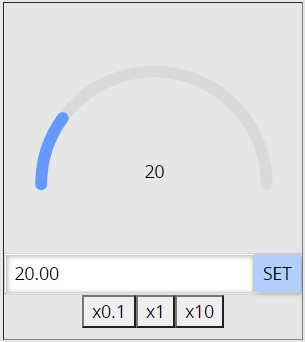
\includegraphics[width=0.4\textwidth]{Tick}
  \caption{Widget contenente una variazione personalizzata della rotazione}
\end{figure}

\section{Utilizzo del Servizio}

Per utilizzare il servizio DialService, occorre importarlo nel costruttore del componente che si sta sviluppando, in questo modo avremo accesso agli eventi che ci consentono di avere notifiche dal Dial.
Inizialmente è necessario creare una voce di Menù che rappresenta il widget all’interno del menù del Dial, così da avere la possibilità di acquisirne il controllo ed avere accesso alle sue funzionalità.
Sotto è riportato un esempio di creazione di una voce di menù per il dial con la relativa aggiunta alla lista di voci di Menu giá presenti.

\vspace{1.0cm}
\begin{lstlisting}[caption={Creazione nuova voce da widget},style=javaScriptCode]
  private createMenuVoice() {
    const dialMenuVoice = this.dialService.dialProxy.createDialMenuItem(
      this.widget.id, this.widget.descriptor.shortText, this.widget.descriptor.icon);
    this.dialService.dialProxy.addItem(dialMenuVoice);
  }
\end{lstlisting} 
\vspace{1.0cm}

Una volta aggiunta la voce di Menu al Dial, essa potrá essere selezionata attraverso il metodo Inkove messo a disposizione dalla classe DialController. Il metodo Invoke per acquisire una voce di menu, potrá essere richiamato sia attraverso il menu contestuale del Dial che compare nello schermo, che tramite un nostro metodo chiamato appunto ManualInvoke che esegue questa azione manualmente, richiamando tramite Web il medesimo metodo, solamente se quella voce di menu é presente tra quelle disponibile nel Dial.
In questo modo, il Widget non dovrá fare altro che mettersi in ascolto del metodo onInvokeEvent, il quale quando richiamato, restituisce una stringa definita “tag”, rappresentante la voce Menu acquisita.
Se quel tag, corrisponde all’id del Widget in ascolto, significa che l’utente ha richiesto il controllo di quel determinato Widget.

\vspace{1.0cm}
\begin{lstlisting}[caption={Ascolto Invoke della voce di menu'},style=javaScriptCode]
  this.dialService.dialFrontendBridge.onInvokeEvent.subscribe(tag => {
        if (tag === this.widget.id) {
          this.isActive = true;
          this.dialService.widget = this.widget.id;
          this.widgetDialStart();
          this.dialService.dialProxy.manualInvoke(this.channels[0].parameter.value);
        }
\end{lstlisting} 
\vspace{1.0cm}

Una volta acquisito il controllo del Widget, bisognerá mettersi in ascolto delle funzioni richiamabili dal Dial, attraverso gli eventEmitter messi a disposizione dalla classe DialFrontndBridge, e implementare il comportamento di quel Widget all’emissione di determinati eventi come la Rotazione o il Click.


\vspace{1.0cm}
\begin{lstlisting}[caption={Ascolto eventi associati alla voce di menu' selezionata},style=javaScriptCode]
const rotation = this.dialService.dialFrontendBridge.onRotationEvent.subscribe(
	({ tag, degree }) => {
      // Azione associata all'evento rotazione del Dial.
      if (tag === this.channels[this.currentChannel].parameter.value) {
        this.setSetterAtIndex(this.currentChannel, 
        parseNumber(degree)* this.moltiplicator
        );
      }
    });

const click = this.dialService.dialFrontendBridge.onClickEvent.subscribe(
	(tag) => {
      // Azione associata all'evento click del Dial.
      if(tag === this.channels[this.currentChannel].parameter.value){
          this.setChannelValue(this.channels[this.currentChannel].parameter.code,
          this.getNumberSetterComponent(this.currentChannel).value);
        }
    });

const pressRot = this.dialService.dialFrontendBridge.onPressedRotationEvent.subscribe(
({ tag, degree }) => {
      if (tag === this.channels[this.currentChannel].parameter.value) {
        this.setSetterAtIndex(
        this.currentChannel, 
        parseNumber(degree) * this.moltiplicator
        );
        this.setChannelValue(this.channels[this.currentChannel].parameter.code,
        this.getNumberSetterComponent(this.currentChannel).value);
      }
    });
\end{lstlisting} 
\vspace{1.0cm}

I metodo sopra implementati, permettono il richiamo di una determinata funzione implementata dall'utilizzatore del servizio, ogni qualvolta venga richiamato un evento presente in DialFrontendBridge come la rotazione o la pressione combinata alla rotazione.
Quest'ultima, permette nel caso dell'acquisizione Widget tramite il contatto del Dial sullo schermo di mantenerne il controllo, evitando il pericolo che nel tratto in cui é il dispositivo si trovi sospeso, possano avvenire chiamate pericolose.

\section{Testing}

Per quanto riguarda i test svolti in ambito UWP abbiamo utilizzato MSTest fornito da Microsoft all’interno di Visual Studio per testare le funzionalitá messe a disposizione dalla classe RadialController.

\subsection{MSTest}
Visual Studio Unit Testing Framework descrive la suite di strumenti di unit test di Microsoft integrata in alcune versioni di Visual Studio 2005 e successive.
Qui sotto sono riportati due tra i vari test implementati nel progetto:
 
\vspace{1.0cm}
\begin{lstlisting}[caption={Test SetMenu},style=javaScriptCode]
    [UITestMethod]
        public void TestSetMenu()
        {
            Assert.IsFalse(radialController.Menu.Items.Count > 0);
            DialMenuItem item1 = dialController.CreateDialMenuItem("tag1", "d", "icon");
            DialMenuItem item2 = dialController.CreateDialMenuItem("tag2", "d", "icon");
            DialMenuItem item3 = dialController.CreateDialMenuItem("tag3", "d", "icon");
            DialMenuItem item4 = dialController.CreateDialMenuItem("tag4", "d", "icon");
            List<DialMenuItem> items = new List<DialMenuItem>();
            items.Add(item1);
            items.Add(item2);
            items.Add(item3);
            items.Add(item4);
            dialController.SetMenu(items);
            Assert.IsTrue(radialController.Menu.Items.Count == 4);
        }
\end{lstlisting} 
\vspace{1.0cm}

\vspace{1.0cm}
\begin{lstlisting}[caption={Test aggiunta voce di Menu'},style=javaScriptCode]
  [UITestMethod]
        public void TestAddItem(){
            Assert.IsFalse(radialController.Menu.Items.Count > 0);
            dialController.AddItem(dialController.CreateDialMenuItem("tag", "d", "icon"));
            Assert.IsTrue(radialController.Menu.Items.Count > 0);
        }
\end{lstlisting} 
\vspace{1.0cm}
